\documentclass[conference]{IEEEtran}

\usepackage[utf8]{inputenc}
\usepackage[T1]{fontenc}
\usepackage[spanish,es-tabla]{babel}
\usepackage{amsmath}
\usepackage[safe]{tipa}
\usepackage{graphicx}
\usepackage{booktabs}
\usepackage{xcolor}
\usepackage{tikz}
\usetikzlibrary{positioning,arrows.meta,fit,calc}
\definecolor{ioc}{HTML}{ECEBE6}
\definecolor{prec}{HTML}{FDE6D6}
\definecolor{convc}{HTML}{CDE2FB}
\definecolor{poolc}{HTML}{FCEBC0}
\definecolor{fcc}{HTML}{CFEFDF}
\usepackage{url}
\usepackage[hidelinks]{hyperref}
\graphicspath{{figuras/}}

\newcommand{\pendiente}[1]{\textcolor{red}{[PENDIENTE: #1]}}
\newcommand{\pend}{\textcolor{red}{??}}

\newcommand{\figtemp}[1]{\fbox{\parbox[c][3cm][c]{0.9\columnwidth}{\centering\small #1}}}

\begin{document}

\title{Reconocimiento de comandos de voz y despliegue móvil con ONNX Runtime Mobile}

\author{
\IEEEauthorblockN{Daniel Zeas Brown}
\IEEEauthorblockA{Escuela de Ingeniería en Computación\\
Instituto Tecnológico de Costa Rica\\
Carné: 2023147474}
\and
\IEEEauthorblockN{Joshua Obando Castro}
\IEEEauthorblockA{Escuela de Ingeniería en Computación\\
Instituto Tecnológico de Costa Rica\\
Carné: 2023130774}
}

\maketitle

\begin{abstract}
Este trabajo presenta un sistema de reconocimiento de 10 comandos de voz (\textit{yes, no, up, down, left, right, on, off, stop, go}) entrenado con el Speech Commands Dataset v0.02 y desplegado en una aplicación Android que realiza la inferencia localmente con ONNX Runtime Mobile. Se compararon dos arquitecturas convolucionales, una variante de LeNet-5 y una red ligera inspirada en MobileNet, entrenadas con datos crudos y con aumento de datos mediante SpecAugment, para un total de 12 experimentos registrados en Weights \& Biases. El mejor modelo fue LeNet-5 con datos aumentados, con una exactitud de validación de 91.7\,\% y 92.2\,\% en test. El modelo se exportó a ONNX incluyendo el cálculo del espectrograma log-mel, se verificó que sus predicciones coinciden con las del modelo original y se integró en una aplicación de navegación por voz tipo \textit{Smart Home} que funciona sin conexión a internet. En una prueba en el teléfono, la aplicación reconoció correctamente 49 de 50 comandos sin ejecutar ninguna acción incorrecta.
\end{abstract}

\begin{IEEEkeywords}
reconocimiento de voz, redes convolucionales, LeNet-5, MobileNet, SpecAugment, ONNX Runtime Mobile, Android
\end{IEEEkeywords}

\section{Introducción}
Las interfaces por voz permiten interactuar con un dispositivo sin usar las manos. En aplicaciones de hogar inteligente, un conjunto pequeño de comandos es suficiente para navegar entre pantallas, confirmar acciones y controlar dispositivos. Ejecutar el reconocimiento directamente en el teléfono evita depender de servicios en la nube, reduce la latencia y protege la privacidad del usuario, pero obliga a usar modelos pequeños y eficientes.

El objetivo de este proyecto es construir la solución completa: preprocesar el audio, entrenar y comparar dos modelos convolucionales, seleccionar el mejor con base en métricas cuantitativas, exportarlo a ONNX e integrarlo en una aplicación móvil navegable por voz.


\section{Estado del arte}
\subsection{Reconocimiento de palabras clave}
El reconocimiento de palabras clave (\textit{keyword spotting}, KWS) consiste en detectar un vocabulario pequeño de palabras en clips cortos de audio. A diferencia del reconocimiento de voz continuo, se plantea como un problema de clasificación y suele ejecutarse en el propio dispositivo, por lo que los modelos deben ser pequeños y rápidos~\cite{zhang2017}.

Tradicionalmente el audio se representa mediante coeficientes o espectrogramas en escala mel, que imitan la resolución en frecuencia del oído humano~\cite{davis1980}. Sainath y Parada~\cite{sainath2015} mostraron que las redes convolucionales (CNN) aplicadas sobre estos espectrogramas superan a las redes totalmente conectadas usadas hasta entonces, con menos parámetros, porque aprovechan la estructura local en tiempo y frecuencia del espectrograma, igual que una CNN lo hace con una imagen.

\subsection{El dataset Speech Commands}
Warden~\cite{warden2018} publicó el Speech Commands Dataset, con decenas de miles de clips de un segundo grabados por miles de personas en condiciones reales y con micrófonos distintos, junto con un modelo convolucional de referencia. Desde entonces es el estándar para comparar modelos de KWS. La mayoría de los trabajos usan una tarea de 12 clases (10 palabras más ``silencio'' y ``desconocido''), por lo que sus resultados no son directamente comparables con la tarea de 10 clases de este proyecto, aunque sí dan una idea del rendimiento esperable.

\subsection{Arquitecturas convolucionales}
\textbf{LeNet-5}~\cite{lecun1998} es una de las primeras CNN exitosas: dos capas convolucionales con submuestreo seguidas de tres capas totalmente conectadas. Fue diseñada para dígitos escritos a mano de $32\times32$ y usa activación tanh y submuestreo por promedio. Las versiones modernas suelen reemplazarlas por ReLU~\cite{nair2010} y \textit{max pooling}, que facilitan el entrenamiento de redes más profundas.

Con el tiempo se buscaron redes más precisas y más eficientes. Tang y Lin~\cite{tang2018} adaptaron las redes residuales (ResNet) a KWS y superaron el 95\,\% de exactitud en Speech Commands. Zhang et al.~\cite{zhang2017} compararon varias arquitecturas para microcontroladores y concluyeron que las CNN con convoluciones separables en profundidad dan el mejor balance entre exactitud, memoria y cómputo.

\textbf{MobileNet}~\cite{howard2017} se basa precisamente en esas convoluciones separables: divide una convolución estándar en una convolución \textit{depthwise}, que aplica un filtro por canal, y una \textit{pointwise} de $1\times1$, que combina los canales. Con filtros de $3\times3$ esto reduce el cómputo entre 8 y 9 veces con una pérdida pequeña de exactitud. MobileNetV2~\cite{sandler2018} añadió bloques residuales invertidos y es una de las arquitecturas más usadas en dispositivos móviles. Trabajos más recientes llevan esta idea más lejos: TC-ResNet~\cite{choi2019} usa convoluciones temporales para lograr inferencia en tiempo real en teléfonos, y BC-ResNet~\cite{kim2021} alcanza 98.7\,\% en Speech Commands v2 con unos 321\,000 parámetros, mientras que su versión más pequeña, con menos de 10\,000, llega a 96.9\,\%. También se han propuesto modelos basados en atención, como el Keyword Transformer~\cite{berg2021}.

\subsection{Aumento de datos para audio}
Como los modelos de KWS deben funcionar con voces, micrófonos y ruidos que no aparecen en el entrenamiento, el aumento de datos es una práctica común. Las técnicas clásicas modifican la señal de audio, por ejemplo cambiando su velocidad~\cite{ko2015}. SpecAugment~\cite{park2019} propuso aplicar el aumento directamente sobre el espectrograma con máscaras en frecuencia y en tiempo y deformación temporal. Es simple, no requiere datos adicionales y mejoró de forma importante los resultados en reconocimiento de voz, por lo que fue la técnica elegida en este trabajo.

\subsection{Despliegue en dispositivos móviles}
Para ejecutar los modelos en el teléfono se usan formatos de intercambio como ONNX, que describen la red como un grafo independiente del framework de entrenamiento. ONNX Runtime Mobile~\cite{onnxruntime} ejecuta estos modelos en Android e iOS sin conexión a internet, lo que reduce la latencia y protege la privacidad del usuario.

\section{Dataset y preprocesamiento}

\subsection{Dataset}
Se utilizó el Speech Commands Dataset v0.02~\cite{warden2018}, que contiene clips de aproximadamente un segundo grabados por miles de personas. Se tomaron únicamente los 10 comandos autorizados, para un total de 38\,546 audios (Tabla~\ref{tab:dataset}).

\begin{table}[htbp]
\caption{Cantidad de audios por comando}
\label{tab:dataset}
\centering
\resizebox{\columnwidth}{!}{%
\begin{tabular}{lr|lr}
\toprule
Comando & Audios & Comando & Audios \\
\midrule
yes   & 4\,044 & right & 3\,778 \\
no    & 3\,941 & on    & 3\,845 \\
up    & 3\,723 & off   & 3\,745 \\
down  & 3\,917 & stop  & 3\,872 \\
left  & 3\,801 & go    & 3\,880 \\
\midrule
\multicolumn{4}{c}{Total: 38\,546} \\
\bottomrule
\end{tabular}}
\end{table}

El conjunto se dividió de forma aleatoria (semilla 42) en 70\,\% entrenamiento (26\,982 audios), 15\,\% validación (5\,781) y 15\,\% prueba (5\,783).

\subsection{Del audio a la imagen: espectrograma log-mel}
Cada audio se carga como señal mono a 16\,kHz con valores en $[-1, 1]$ y se ajusta a exactamente 1 segundo (16\,000 muestras): los clips más cortos se rellenan con ceros al final y los más largos se recortan. Luego se calcula:

\begin{enumerate}
  \item \textbf{Espectrograma mel} con ventanas de 400 muestras (25\,ms), salto de 160 muestras (10\,ms) y 80 bandas mel. El resultado es una matriz de $80 \times 101$ (frecuencia $\times$ tiempo).
  \item \textbf{Conversión a decibeles} (log-mel) con un rango dinámico máximo de 80\,dB. La escala logarítmica comprime el rango de energías y se parece más a cómo percibe el oído humano.
  \item \textbf{Normalización global}: $x' = (x - \mu)/\sigma$, con la media $\mu$ y desviación $\sigma$ calculadas sobre todo el dataset.
\end{enumerate}

Así cada audio se convierte en una imagen de un canal de $1 \times 80 \times 101$, que es la entrada de las redes convolucionales (Fig.~\ref{fig:espectro}).

\begin{figure*}[htbp]
\centering
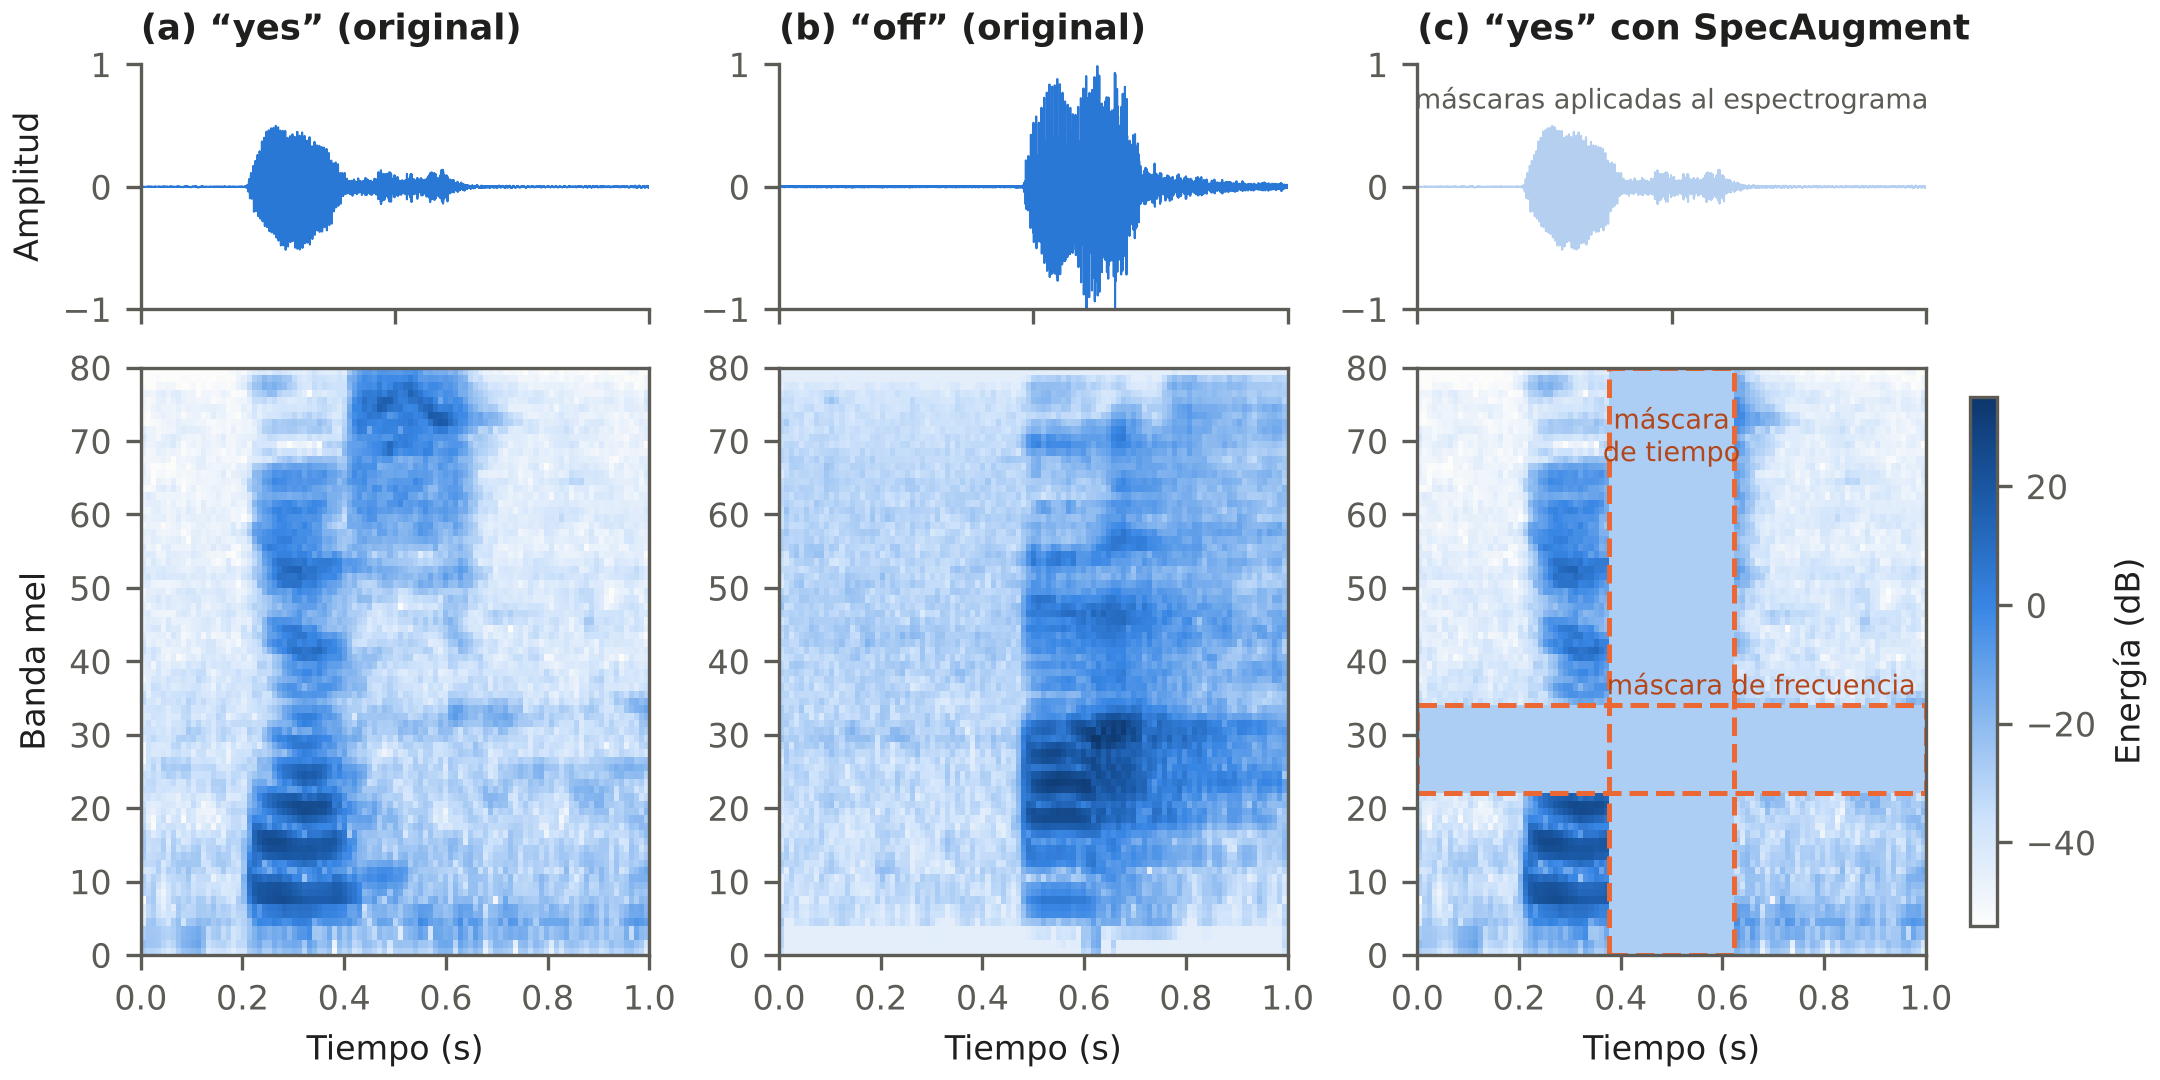
\includegraphics[width=0.9\textwidth]{espectrogramas.png}
\caption{Dos audios del dataset: forma de onda (arriba) y espectrograma log-mel de $80\times101$ que recibe la red (abajo). En (a), la /s/ final de ``yes'' aparece como energía en las bandas altas (60--80); en (b), ``off'' concentra su energía en las bandas bajas. (c) muestra el mismo ``yes'' tras aplicar SpecAugment: una máscara de frecuencia y una de tiempo reemplazan esas regiones por el valor medio. El modelo final clasifica (a) como ``yes'' con 100\,\% de confianza y (b) como ``off'' con 94\,\%.}
\label{fig:espectro}
\end{figure*}

\subsection{Aumento de datos}
Para el conjunto \textit{aumentado} se aplicó SpecAugment~\cite{park2019} sobre el espectrograma, de forma aleatoria en cada época y solo en entrenamiento:

\begin{itemize}
  \item \textbf{Máscara de frecuencia}: oculta hasta 15 bandas mel consecutivas.
  \item \textbf{Máscara de tiempo}: oculta hasta 35 cuadros consecutivos (350\,ms).
\end{itemize}

La Fig.~\ref{fig:espectro}c muestra un ejemplo. Estas máscaras simulan ruido, partes de la palabra mal captadas y diferencias entre micrófonos, lo que obliga a la red a no depender de una sola región del espectrograma. Los conjuntos de validación y prueba nunca reciben aumento.

\section{Arquitecturas}
Ambos modelos se implementaron manualmente con \texttt{torch.nn}.

\subsection{Modelo A: LeNet-5}
Se partió de LeNet-5~\cite{lecun1998} y se adaptó la entrada a espectrogramas de $1 \times 80 \times 101$. Las dimensiones de cada capa se muestran en la Tabla~\ref{tab:lenet}. Como la entrada no es de $32 \times 32$ como en el original, la salida de la segunda capa de submuestreo queda en $16 \times 17 \times 22$, y por eso la primera capa totalmente conectada recibe 5\,984 valores.

\begin{table}[htbp]
\caption{Dimensiones del Modelo A (LeNet-5)}
\label{tab:lenet}
\centering
\resizebox{\columnwidth}{!}{%
\begin{tabular}{llr}
\toprule
Capa & Salida & Parámetros \\
\midrule
Entrada              & $1 \times 80 \times 101$  & -- \\
Conv $5\times5$, 6 filtros + ReLU   & $6 \times 76 \times 97$   & 156 \\
MaxPool $2\times2$   & $6 \times 38 \times 48$   & -- \\
Conv $5\times5$, 16 filtros + ReLU  & $16 \times 34 \times 44$  & 2\,416 \\
MaxPool $2\times2$   & $16 \times 17 \times 22$  & -- \\
Aplanado             & 5\,984                    & -- \\
FC + ReLU            & 120                       & 718\,200 \\
FC + ReLU            & 84                        & 10\,164 \\
FC (logits)          & 10                        & 850 \\
\midrule
\multicolumn{2}{l}{Total} & 731\,786 \\
\bottomrule
\end{tabular}}
\end{table}

\textbf{Modificación respecto al LeNet-5 clásico.} El LeNet-5 original usa activación tanh y submuestreo por promedio (\textit{average pooling}). En este trabajo se usó \textbf{ReLU} y \textbf{max pooling}. La función ReLU evita la saturación de tanh, que reduce el gradiente y hace más lento el entrenamiento, y max pooling conserva la activación más fuerte de cada región, lo que en espectrogramas ayuda a mantener los picos de energía característicos de cada palabra. Además, ReLU es más barata de calcular que tanh, y eso cuenta cuando el modelo corre en un teléfono. En las pruebas, esta variante fue la que alcanzó la mayor exactitud de todos los modelos (Sección~VI).

\begin{figure*}[htbp]
\centering
\resizebox{\textwidth}{!}{%
\begin{tikzpicture}[blk/.style={draw=black!55, rounded corners=2pt, align=center, font=\scriptsize, minimum height=14mm, text width=16mm, inner sep=2pt},
  io/.style={blk, fill=ioc}, pre/.style={blk, fill=prec}, conv/.style={blk, fill=convc},
  pool/.style={blk, fill=poolc}, fc/.style={blk, fill=fcc},
  flecha/.style={-{Stealth[length=1.8mm]}, black!60, thick}, node distance=2.5mm]
\node[io] (in) {Audio\\$[16000]$\\16\,kHz};
\node[pre, right=of in] (mel) {Log-mel\\normalizado\\$1{\times}80{\times}101$};
\node[conv, right=of mel] (c1) {Conv $5{\times}5$\\6 filtros\\+ ReLU\\$6{\times}76{\times}97$};
\node[pool, right=of c1] (p1) {MaxPool\\$2{\times}2$\\$6{\times}38{\times}48$};
\node[conv, right=of p1] (c2) {Conv $5{\times}5$\\16 filtros\\+ ReLU\\$16{\times}34{\times}44$};
\node[pool, right=of c2] (p2) {MaxPool\\$2{\times}2$\\$16{\times}17{\times}22$};
\node[io, right=of p2] (fl) {Aplanado\\5\,984};
\node[fc, right=of fl] (f1) {FC + ReLU\\120};
\node[fc, right=of f1] (f2) {FC + ReLU\\84};
\node[fc, right=of f2] (f3) {FC\\10 logits};
\foreach \x/\y in {in/mel, mel/c1, c1/p1, p1/c2, c2/p2, p2/fl, fl/f1, f1/f2, f2/f3} \draw[flecha] (\x) -- (\y);
\end{tikzpicture}}
\caption{Arquitectura del Modelo A (LeNet-5). El bloque naranja es el preprocesamiento, que va incluido dentro del modelo exportado a ONNX. En cada bloque se indica la forma de su salida.}
\label{fig:lenet}
\end{figure*}

\subsection{Modelo B: red ligera inspirada en MobileNet}
El Modelo B se basa en MobileNet~\cite{howard2017}. Inicia con una convolución estándar y sigue con tres bloques de convolución separable en profundidad: una convolución \textit{depthwise} de $3\times3$ (un filtro por canal) seguida de una \textit{pointwise} de $1\times1$ que combina los canales, con normalización por lotes y ReLU. Cada bloque reduce a la mitad la resolución (paso 2) y duplica los canales. Al final, un \textit{pooling} promedio adaptativo deja un vector de 128 valores sin importar el tamaño de la entrada (Tabla~\ref{tab:mobilenet}).

\begin{table}[htbp]
\caption{Dimensiones del Modelo B (MobileNet)}
\label{tab:mobilenet}
\centering
\resizebox{\columnwidth}{!}{%
\begin{tabular}{llr}
\toprule
Capa & Salida & Parámetros \\
\midrule
Entrada                          & $1 \times 80 \times 101$  & -- \\
Conv $3\times3$/2 + BN + ReLU    & $16 \times 40 \times 51$  & 192 \\
Bloque separable /2              & $32 \times 20 \times 26$  & 768 \\
Bloque separable /2              & $64 \times 10 \times 13$  & 2\,560 \\
Bloque separable /2              & $128 \times 5 \times 7$   & 9\,216 \\
Pooling promedio adaptativo      & 128                       & -- \\
FC (logits)                      & 10                        & 1\,290 \\
\midrule
\multicolumn{2}{l}{Total} & 14\,026 \\
\bottomrule
\end{tabular}}
\end{table}

El Modelo B tiene unas 52 veces menos parámetros que el Modelo A. En una aplicación móvil esa diferencia pesa.

\begin{figure*}[htbp]
\centering
\resizebox{\textwidth}{!}{%
\begin{tikzpicture}[blk/.style={draw=black!55, rounded corners=2pt, align=center, font=\scriptsize, minimum height=14mm, text width=16mm, inner sep=2pt},
  io/.style={blk, fill=ioc}, pre/.style={blk, fill=prec}, conv/.style={blk, fill=convc},
  pool/.style={blk, fill=poolc}, fc/.style={blk, fill=fcc},
  flecha/.style={-{Stealth[length=1.8mm]}, black!60, thick}, node distance=2.5mm]
\node[io] (in) {Audio\\$[16000]$\\16\,kHz};
\node[pre, right=of in] (mel) {Log-mel\\normalizado\\$1{\times}80{\times}101$};
\node[conv, right=of mel] (c1) {Conv $3{\times}3$/2\\16 filtros\\+ BN + ReLU\\$16{\times}40{\times}51$};
\node[conv, right=of c1, fill=convc!60!white, draw=black!70, very thick] (d1) {Bloque\\separable /2\\$32{\times}20{\times}26$};
\node[conv, right=of d1, fill=convc!60!white, draw=black!70, very thick] (d2) {Bloque\\separable /2\\$64{\times}10{\times}13$};
\node[conv, right=of d2, fill=convc!60!white, draw=black!70, very thick] (d3) {Bloque\\separable /2\\$128{\times}5{\times}7$};
\node[pool, right=of d3] (gap) {Pooling\\promedio\\adaptativo\\128};
\node[fc, right=of gap] (fc) {FC\\10 logits};
\foreach \x/\y in {in/mel, mel/c1, c1/d1, d1/d2, d2/d3, d3/gap, gap/fc} \draw[flecha] (\x) -- (\y);
\node[conv, below=9mm of c1, xshift=12mm] (dw) {Depthwise\\$3{\times}3$, paso 2\\(1 filtro\\por canal)};
\node[conv, right=of dw] (pw) {Pointwise\\$1{\times}1$\\(combina\\canales)};
\node[blk, right=of pw, fill=white] (bn) {BatchNorm};
\node[blk, right=of bn, fill=white] (re) {ReLU};
\foreach \x/\y in {dw/pw, pw/bn, bn/re} \draw[flecha] (\x) -- (\y);
\node[draw=black!70, very thick, dashed, rounded corners=3pt, inner sep=3mm, fit=(dw)(re),
      label={[font=\scriptsize\bfseries]east:\ Bloque separable en profundidad}] (det) {};
\draw[black!50, dashed] (d2.south) -- (det.north -| d2.south);
\end{tikzpicture}}
\caption{Arquitectura del Modelo B (MobileNet). Cada bloque separable (contorno grueso) sigue la estructura del recuadro inferior: reduce a la mitad la resolución y duplica los canales.}
\label{fig:mobilenet}
\end{figure*}

\section{Entrenamiento}
Todos los modelos se entrenaron con entropía cruzada como función de pérdida y el optimizador Adam, con semilla fija (42) para que los resultados sean reproducibles. En cada época se evaluó el conjunto de validación y se guardaron los pesos de la época con menor pérdida de validación. Las métricas se registraron en Weights \& Biases.

Para cada una de las cuatro combinaciones (modelo $\times$ datos) se hicieron tres entrenamientos con distintos hiperparámetros, para un total de 12 (Tabla~\ref{tab:corridas}).

\begin{table*}[htbp]
\caption{Resultados de validación de los 12 entrenamientos (época con menor pérdida de validación)}
\label{tab:corridas}
\centering
\begin{tabular}{llcccccc}
\toprule
Modelo & Datos & Exp. & LR & Batch & Épocas & Mejor época & val\_loss / val\_acc \\
\midrule
A (LeNet-5)   & Base       & 1 & 0.001  & 64  & 15 & 4  & 0.349 / 89.0\,\% \\
A (LeNet-5)   & Base       & 2 & 0.0005 & 128 & 15 & 6  & 0.395 / 86.5\,\% \\
A (LeNet-5)   & Base       & 3 & 0.001  & 32  & 10 & 4  & \textbf{0.347 / 89.4\,\%} \\
\midrule
A (LeNet-5)   & Aumentado  & 1 & 0.001  & 64  & 15 & 12 & \textbf{0.243 / 91.7\,\%} \\
A (LeNet-5)   & Aumentado  & 2 & 0.0005 & 128 & 15 & 14 & 0.341 / 87.9\,\% \\
A (LeNet-5)   & Aumentado  & 3 & 0.001  & 32  & 10 & 8  & 0.272 / 90.9\,\% \\
\midrule
B (MobileNet) & Base       & 1 & 0.001  & 64  & 15 & 13 & \textbf{0.370 / 88.3\,\%} \\
B (MobileNet) & Base       & 2 & 0.0005 & 128 & 15 & 14 & 0.553 / 83.3\,\% \\
B (MobileNet) & Base       & 3 & 0.001  & 32  & 10 & 8  & 0.382 / 87.9\,\% \\
\midrule
B (MobileNet) & Aumentado  & 1 & 0.001  & 64  & 15 & 12 & 0.445 / 85.8\,\% \\
B (MobileNet) & Aumentado  & 2 & 0.0005 & 128 & 15 & 14 & 0.832 / 72.0\,\% \\
B (MobileNet) & Aumentado  & 3 & 0.001  & 32  & 10 & 9  & \textbf{0.423 / 86.4\,\%} \\
\bottomrule
\end{tabular}
\end{table*}

\subsection{Análisis de sobreajuste y subajuste}
Las curvas de pérdida y exactitud están en las Fig.~\ref{fig:curvas} y~\ref{fig:exactitud}. En LeNet-5 con datos crudos el sobreajuste es claro. La pérdida de entrenamiento llega a 0.03, mientras que la de validación toca su mínimo en la época 4 y después sube hasta 0.62 en el Exp.~1. Por eso guardamos los pesos de la época con menor pérdida de validación y no los de la última.

Con SpecAugment ese comportamiento desaparece: la pérdida de validación de LeNet-5 baja hasta el final y la mejor exactitud sube de 89.4\,\% a 91.7\,\%.

MobileNet se comporta distinto. Sus curvas de validación todavía bajaban cuando terminó el entrenamiento, una señal de subajuste. Con aumento de datos su pérdida de entrenamiento queda incluso por encima de la de validación, porque las máscaras solo se aplican al entrenar.

Los tres experimentos de cada combinación cambiaban a la vez la tasa de aprendizaje, el tamaño de lote y el número de épocas, así que sus efectos no se pueden separar del todo. Contar las actualizaciones de los pesos ayuda a compararlos. Con 26\,982 audios de entrenamiento, el Exp.~1 (lote de 64, 15 épocas) hace unas 6\,300 actualizaciones, el Exp.~2 (lote de 128, 15 épocas) unas 3\,200 y el Exp.~3 (lote de 32, 10 épocas) unas 8\,400. El Exp.~2 tenía además la tasa más baja, 0.0005, la mitad del valor por defecto de Adam. Fue el peor en las cuatro combinaciones: con la mitad de la tasa y la mitad de las actualizaciones del Exp.~1, no alcanzó a converger. En LeNet-5, 15 épocas fueron suficientes; en MobileNet la pérdida seguía bajando, y habría necesitado más.

\begin{figure*}[htbp]
\centering
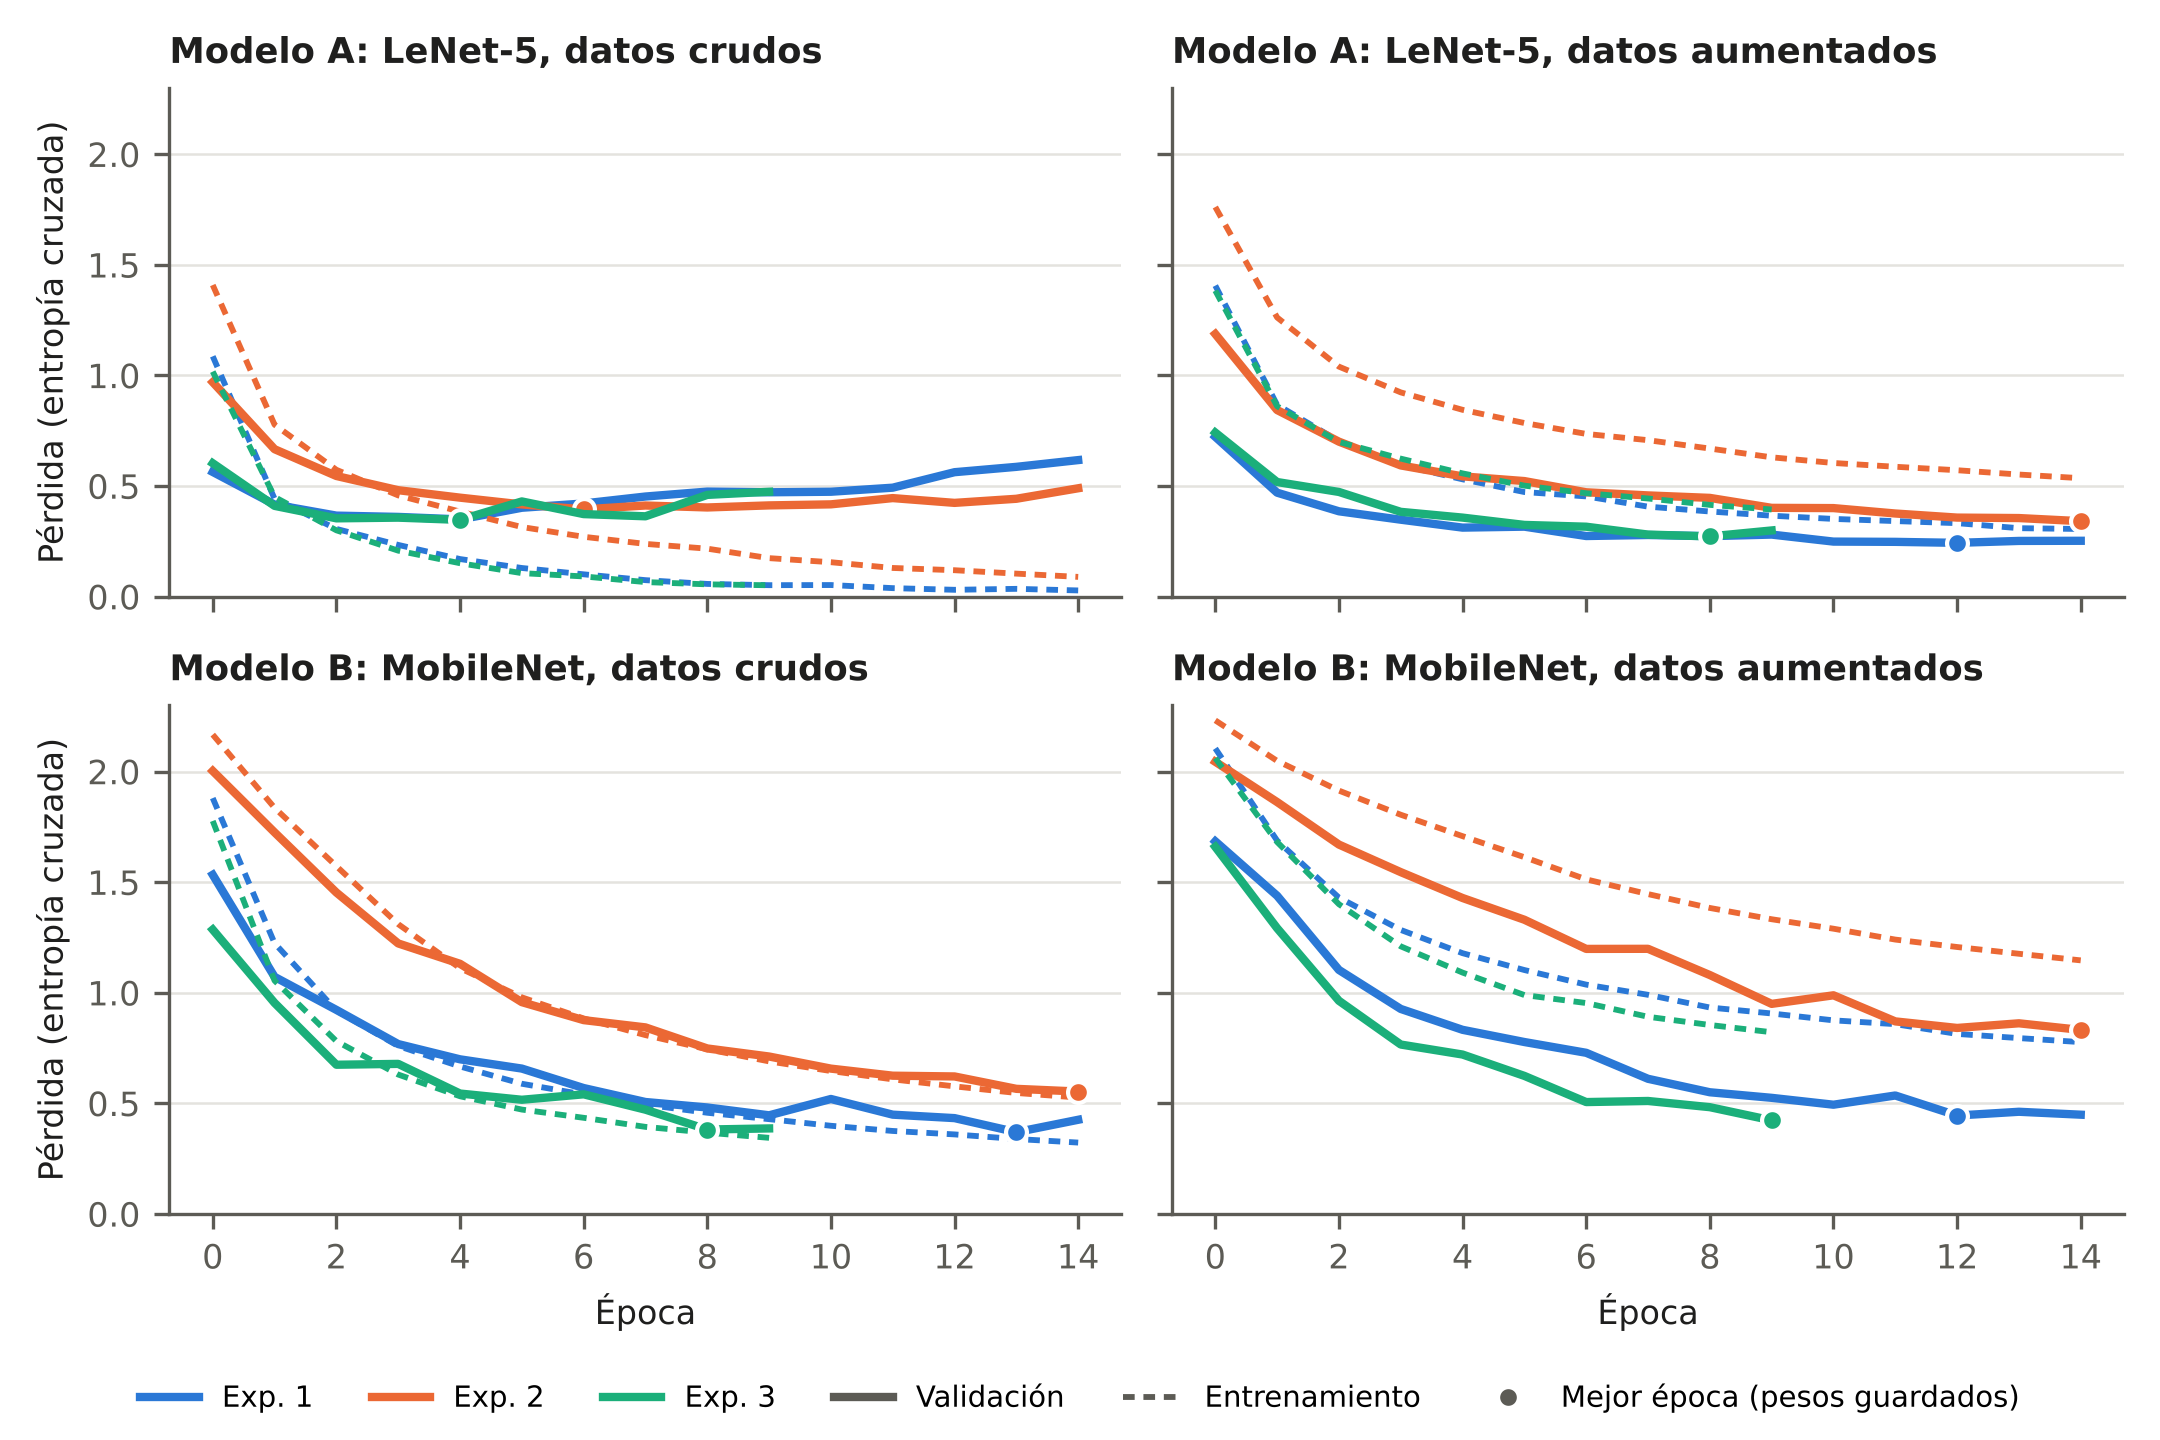
\includegraphics[width=0.95\textwidth]{curvas_perdida.png}
\caption{Pérdida de entrenamiento (punteada) y de validación (sólida) de los 12 entrenamientos, con los datos exportados de Weights \& Biases. El punto marca la época con menor pérdida de validación, cuyos pesos se guardaron.}
\label{fig:curvas}
\end{figure*}

\begin{figure*}[htbp]
\centering
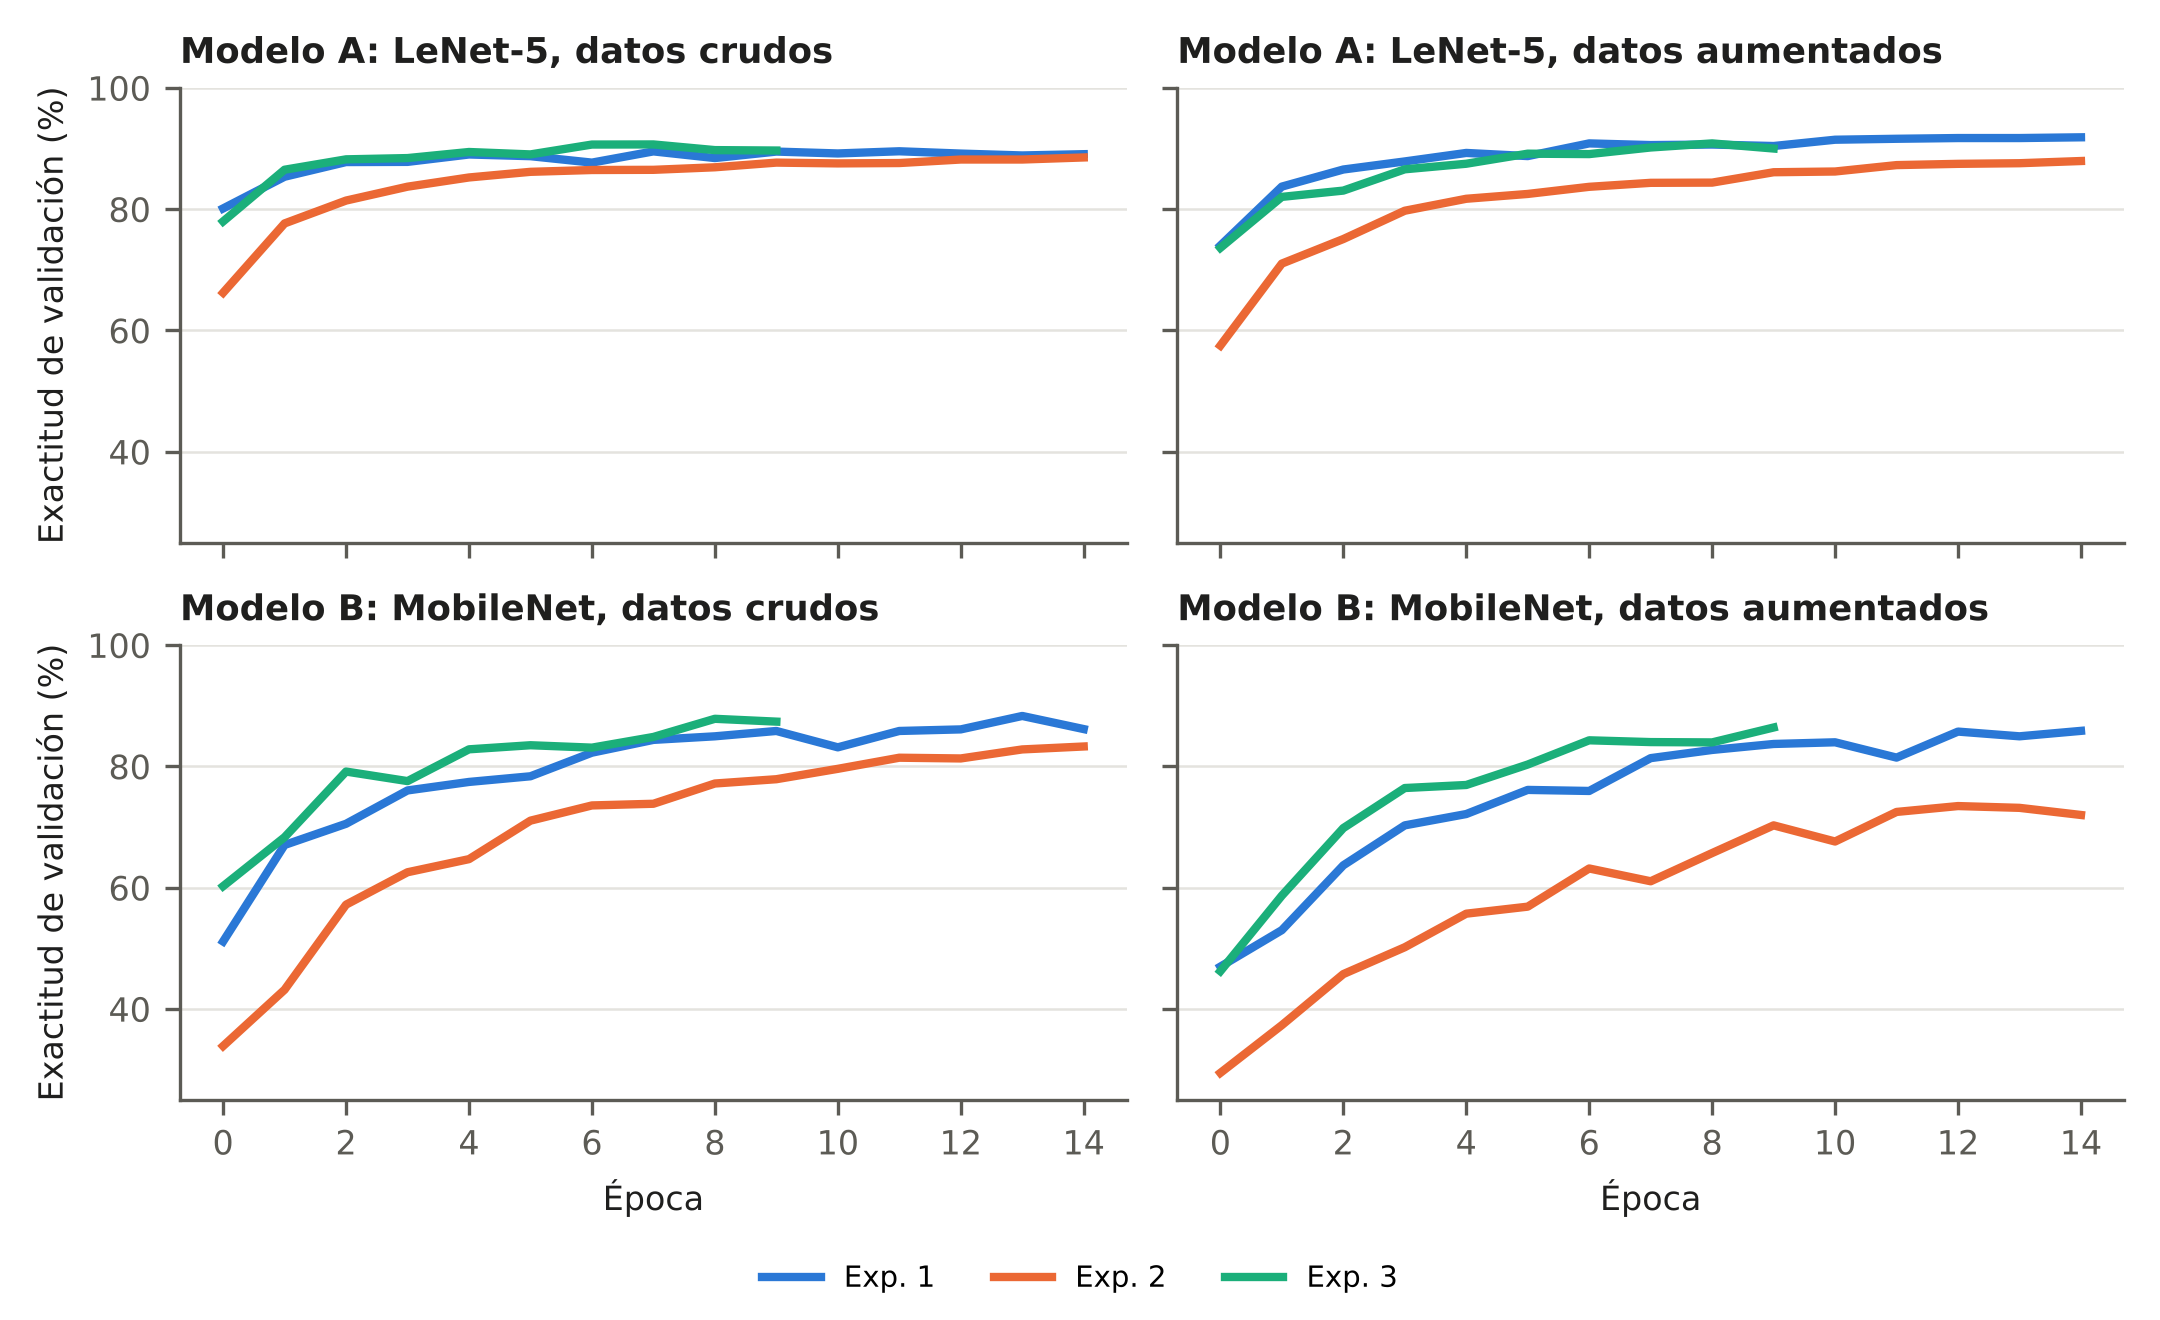
\includegraphics[width=0.95\textwidth]{curvas_exactitud.png}
\caption{Exactitud de validación por época de los 12 entrenamientos.}
\label{fig:exactitud}
\end{figure*}

\section{Evaluación en test y selección del modelo}
Los mejores modelos de cada combinación se evaluaron sobre el conjunto de prueba, que no se usó en ningún momento del entrenamiento ni de la selección de hiperparámetros (Tabla~\ref{tab:test}).

\begin{table}[htbp]
\caption{Resultados en el conjunto de prueba}
\label{tab:test}
\centering
\resizebox{\columnwidth}{!}{%
\begin{tabular}{lccr}
\toprule
Modelo & Exactitud & F1 & Parámetros \\
\midrule
A / Base (Exp.~3)       & 89.8\,\% & 0.898 & 731\,786 \\
\textbf{A / Aumentado (Exp.~1)}  & \textbf{92.2\,\%} & \textbf{0.922} & 731\,786 \\
B / Base (Exp.~1)       & 88.8\,\% & 0.888 & 14\,026 \\
B / Aumentado (Exp.~3)  & 85.8\,\% & 0.859 & 14\,026 \\
\bottomrule
\end{tabular}}
\end{table}

\begin{figure*}[htbp]
\centering
\includegraphics[width=0.92\textwidth]{confusion_lenet_pares.png}
\caption{(a) Matriz de confusión en test del modelo final, LeNet-5 aumentado, en número de audios (solo se anotan los valores de 5 o más). (b) Los ocho pares con más errores sumando los dos modelos, comparando LeNet-5 aumentado con MobileNet base. Los datos se exportaron de Weights \& Biases.}
\label{fig:confusion}
\end{figure*}

\subsection{Análisis de las matrices de confusión}
La mayoría de los errores caen en unos pocos pares de palabras (Fig.~\ref{fig:confusion}). En LeNet-5 la palabra con menos aciertos es ``no'' (85.1\,\%): 42 de sus 569 audios de prueba se clasificaron como ``go'' y 33 como ``down''. ``No'' y ``go'' comparten el diptongo /o\textipa{U}/ y solo cambia la consonante inicial, que dura muy poco. ``Down'' tiene otro diptongo, /a\textipa{U}/, pero también cierra en /\textipa{U}/, y su consonante inicial /d/ es una oclusiva sonora igual que la /g/ de ``go''; eso puede explicar que ``go'' y ``down'' también se confundan entre sí (27 audios de ``go'' se predijeron como ``down''). La otra confusión frecuente en LeNet-5 es ``off'' con ``on'' (25 audios) y con ``up'' (20), tres palabras muy cortas con vocales cercanas.

En MobileNet la palabra con menos aciertos es ``go'' (81.1\,\%), seguida de ``no'' (82.8\,\%), y aparecen confusiones que LeNet-5 casi no tiene, como ``right''$\rightarrow$``left'' (25 audios) y ``stop''$\rightarrow$``up'' (28).

Las palabras que LeNet-5 reconoce mejor son ``right'' (97.7\,\%) y ``yes'' (97.3\,\%). En el espectrograma de ``yes'' la /s/ final se ve como energía en las bandas altas (Fig.~\ref{fig:espectro}a).

Con este modelo esos errores no se pueden eliminar del todo, así que en la aplicación importa qué pasa cuando ocurren. El umbral de 70\,\% y la pantalla de confirmación, que estaban en el diseño desde el inicio, evitan que una confusión apague un dispositivo o detenga una rutina sin que el usuario lo quiera.

\subsection{Comparación de modelos finales}
El modelo seleccionado para la aplicación fue \textbf{LeNet-5 con datos aumentados (Exp.~1)}, por tener la menor pérdida y la mayor exactitud de validación. En test obtuvo 92.2\,\% de exactitud y un F1 de 0.922. En validación había tenido 91.7\,\%, así que el resultado se mantuvo con audios que el modelo no había visto. Como las clases están balanceadas, la exactitud y el F1 son prácticamente iguales en los cuatro modelos.

El aumento de datos tuvo efectos opuestos en las dos arquitecturas: en LeNet-5 subió la exactitud en test de 89.8\,\% a 92.2\,\% al reducir el sobreajuste, mientras que en MobileNet la bajó de 88.8\,\% a 85.8\,\%. MobileNet, con muchos menos parámetros, ya estaba en subajuste, y las máscaras de SpecAugment hicieron la tarea de entrenamiento aún más difícil sin darle más épocas para compensar.

El mejor MobileNet (Base) obtuvo 3.4 puntos menos de exactitud en test, pero con 52 veces menos parámetros. Para este proyecto se priorizó la exactitud, porque el modelo de LeNet-5 ocupa solo 3\,MB y en el teléfono de prueba responde sin una demora perceptible después de la grabación. En un dispositivo con menos recursos, o con escucha continua, MobileNet sería la opción más eficiente.

\section{Exportación a ONNX}
Para que la aplicación solo tenga que enviar audio crudo, el modelo se exportó dentro de un \textit{wrapper} que incluye todo el preprocesamiento: espectrograma mel, conversión a decibeles y normalización con la media y desviación del entrenamiento. El contrato del modelo es:

\begin{itemize}
  \item \textbf{Entrada} \texttt{audio\_in}: tensor \texttt{float32} de forma $[16000]$, audio mono a 16\,kHz con valores en $[-1, 1]$.
  \item \textbf{Salida} \texttt{logits\_out}: tensor de forma $[1, 10]$ con los logits en el orden \textit{yes, no, up, down, left, right, on, off, stop, go}.
\end{itemize}

El modelo se exportó con \texttt{torch.onnx.export} (opset 18) en un único archivo de 3\,MB.

\subsection{Validación del modelo exportado}
Se compararon las salidas del modelo en PyTorch y del archivo ONNX (ejecutado con ONNX Runtime) sobre 3\,000 audios del dataset (300 por comando), cargados igual que en la aplicación:

\begin{itemize}
  \item Las predicciones coincidieron en \textbf{3\,000 de 3\,000} casos.
  \item La diferencia máxima entre logits fue de 0.0063, atribuible a diferencias de precisión numérica entre ambas librerías.
\end{itemize}

\subsection{Problema encontrado durante la exportación}
La primera versión del notebook con la exportación a ONNX se subió al repositorio el 9 de octubre, y el 11 integramos ese modelo en la aplicación. Cargaba sin errores, pero algo no cuadraba: con un segundo de puro silencio respondía ``go''. El 12, al revisar el notebook, encontramos dos diferencias entre el modelo exportado y el entrenado. La celda de exportación volvía a definir LeNet-5 con tanh y \textit{average pooling}, cuando el entrenamiento había usado ReLU y \textit{max pooling}; los pesos cargaban sin error porque los nombres y tamaños de las capas eran iguales. Además, el \textit{wrapper} calculaba el espectrograma mel pero se saltaba la conversión a decibeles y la normalización. Eso también explicaba que la evaluación en test diera 15\,\%, cercano al azar, porque esa celda se ejecutaba después de la redefinición.

El 13 por la tarde, todavía con ese modelo, hicimos la primera prueba en el teléfono: al decir ``down'' respondió ``go'' con 39\,\% de confianza. Esa noche quedó en el repositorio la corrección, que reutiliza la misma clase del entrenamiento, agrega la conversión a decibeles y la normalización al \textit{wrapper}, y suma la comparación PyTorch--ONNX de la sección anterior, que en la primera versión no existía.

\section{Aplicación móvil}
La aplicación se desarrolló para Android en Kotlin con Jetpack Compose (Android 7.0 o superior). La inferencia se realiza localmente con ONNX Runtime Mobile 1.27.0: la aplicación no usa servicios externos y no solicita el permiso de internet.

\subsection{Pantallas}
Siguiendo el prototipo del enunciado, la aplicación tiene cuatro pantallas (Fig.~\ref{fig:app}):

\begin{itemize}
  \item \textbf{Inicio}: tarjetas de Luces, Ventilador, TV y Rutinas en una cuadrícula de $2\times2$. \textit{up/down/left/right} mueven el foco y \textit{yes} abre la tarjeta.
  \item \textbf{Dispositivo}: \textit{on/off} encienden o apagan, \textit{yes} confirma la opción resaltada y \textit{no} regresa.
  \item \textbf{Rutinas}: \textit{up/down} se mueven entre rutinas, \textit{go} inicia, \textit{stop} detiene y \textit{no} regresa.
  \item \textbf{Confirmación}: aparece antes de acciones sensibles (apagar un dispositivo o detener una rutina). \textit{yes} ejecuta y \textit{no} cancela.
\end{itemize}

Toda la lógica pasa por una única función, \texttt{handle(comando)}, que decide qué hacer según la pantalla actual. La llaman tanto el modelo como unos botones de comandos simulados, que se mantienen como modo de prueba.

\begin{figure*}[htbp]
\centering
\begin{minipage}[t]{0.23\textwidth}\centering
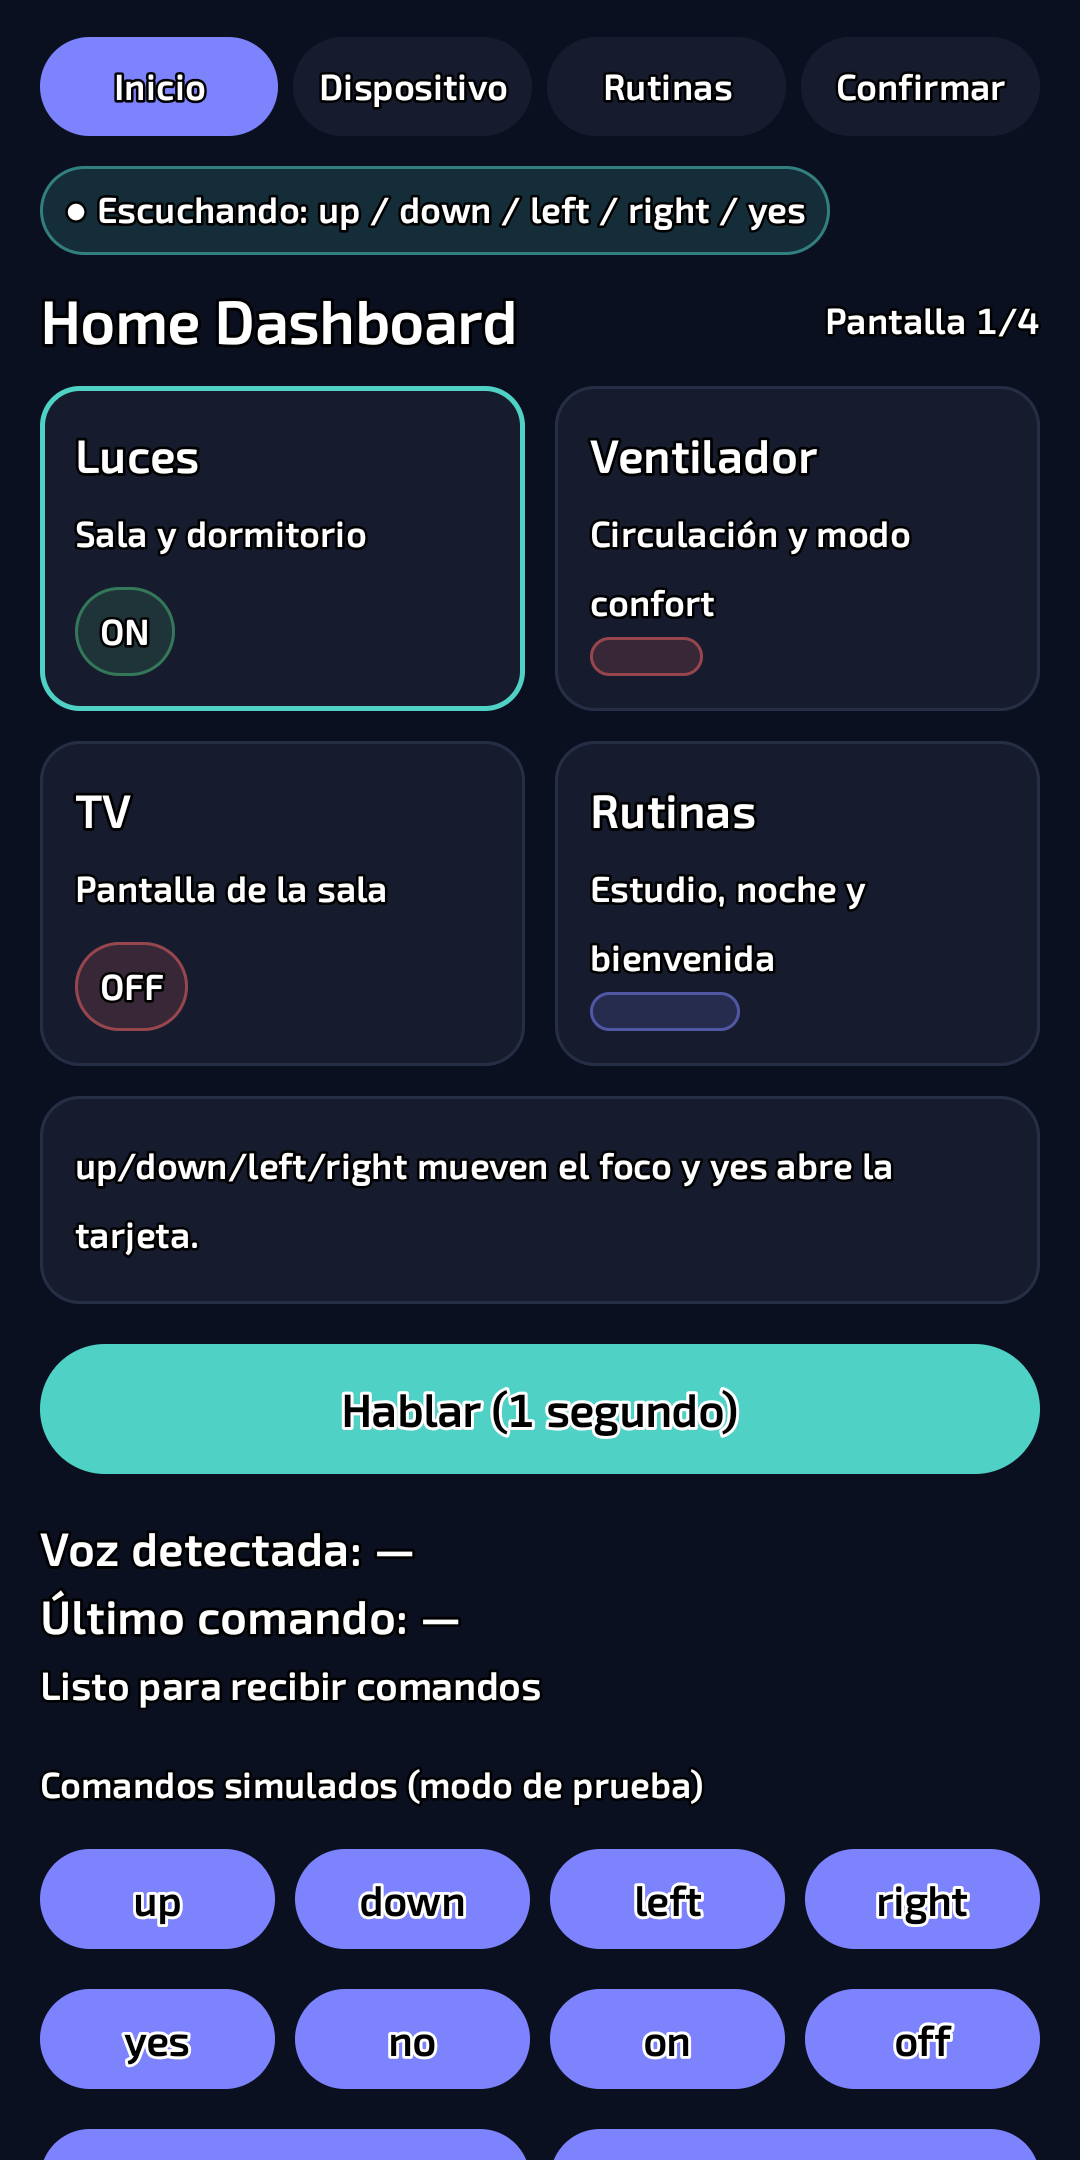
\includegraphics[width=\textwidth]{app_inicio.png}\\[2pt]{\footnotesize (a) Inicio}
\end{minipage}\hfill
\begin{minipage}[t]{0.23\textwidth}\centering
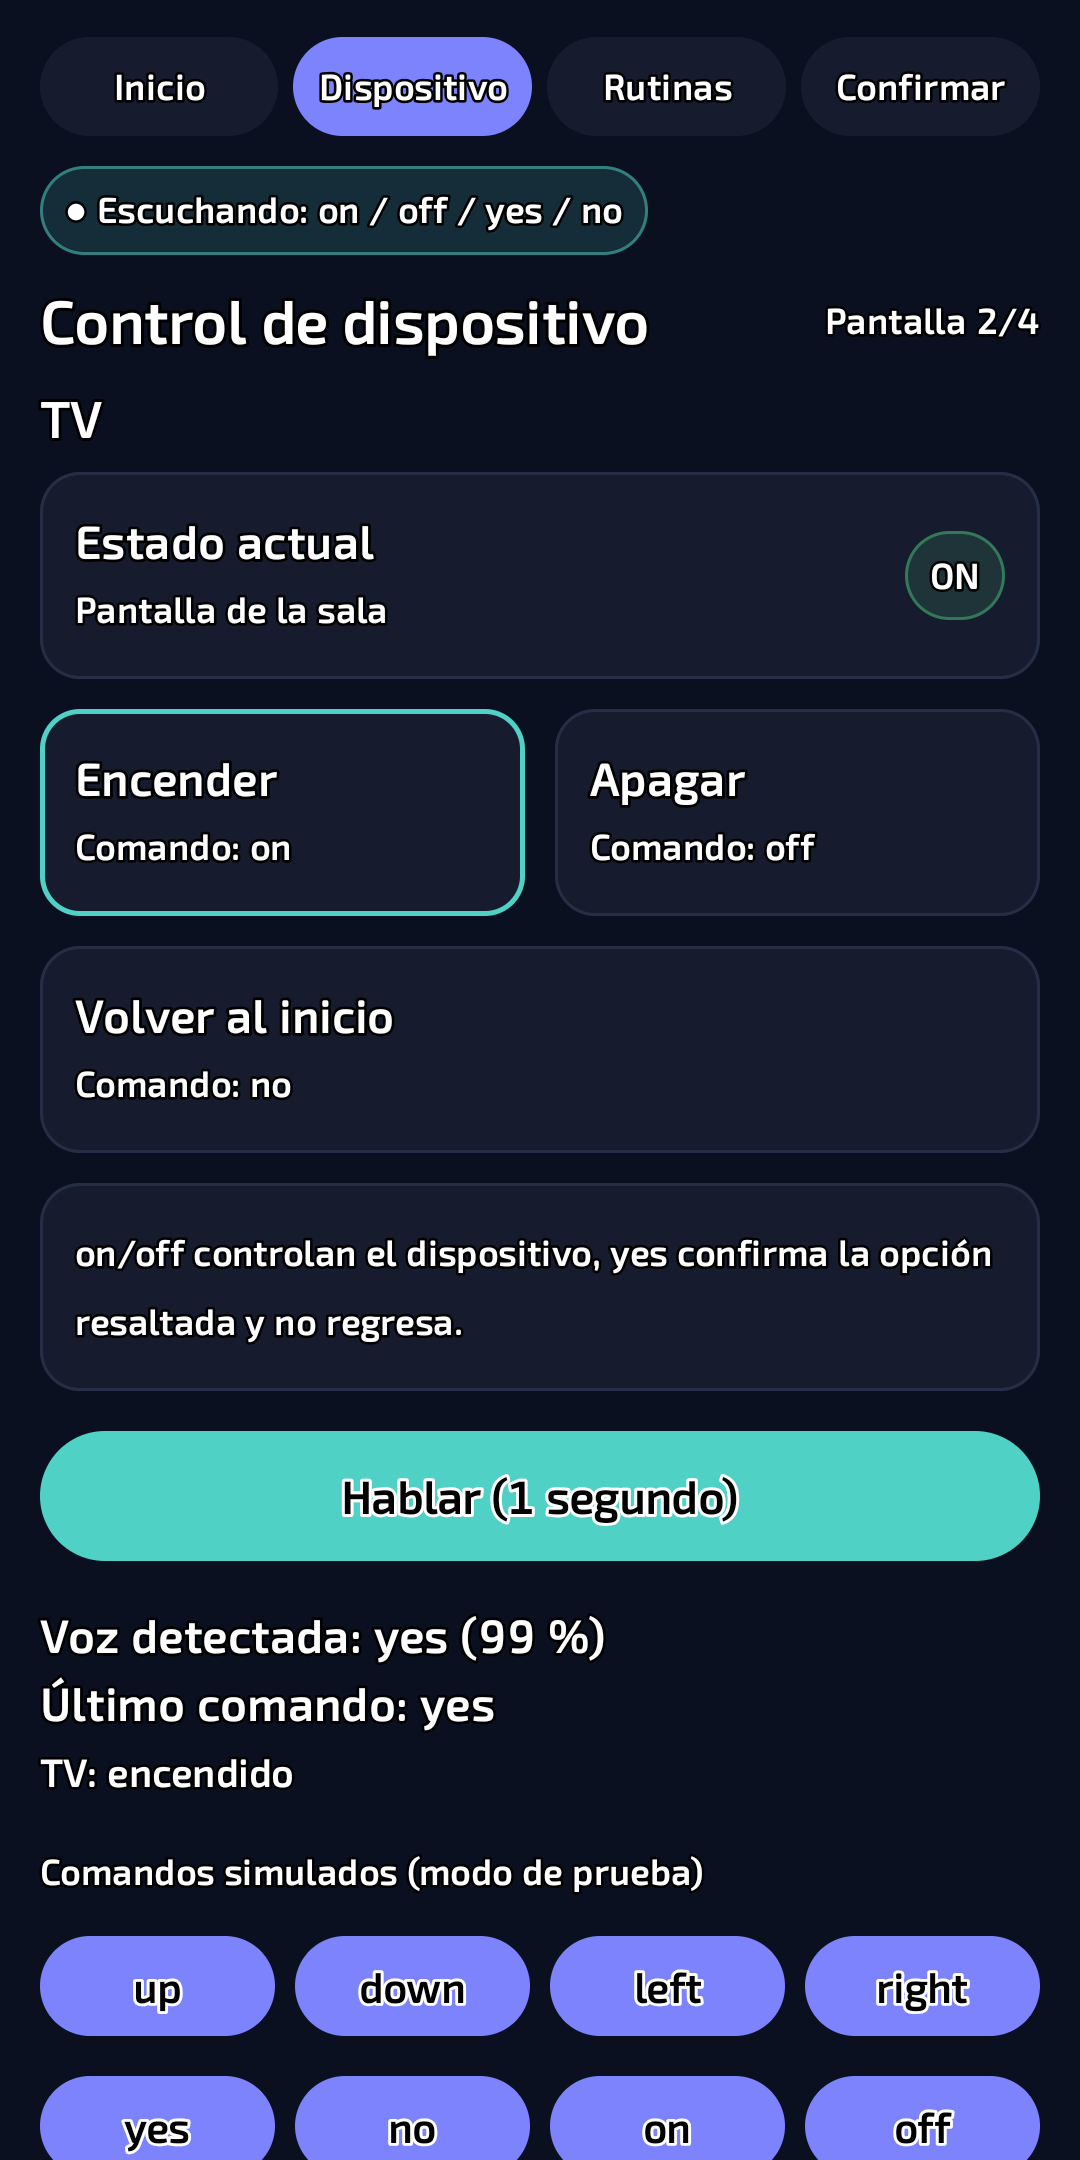
\includegraphics[width=\textwidth]{app_dispositivo.png}\\[2pt]{\footnotesize (b) Dispositivo}
\end{minipage}\hfill
\begin{minipage}[t]{0.23\textwidth}\centering
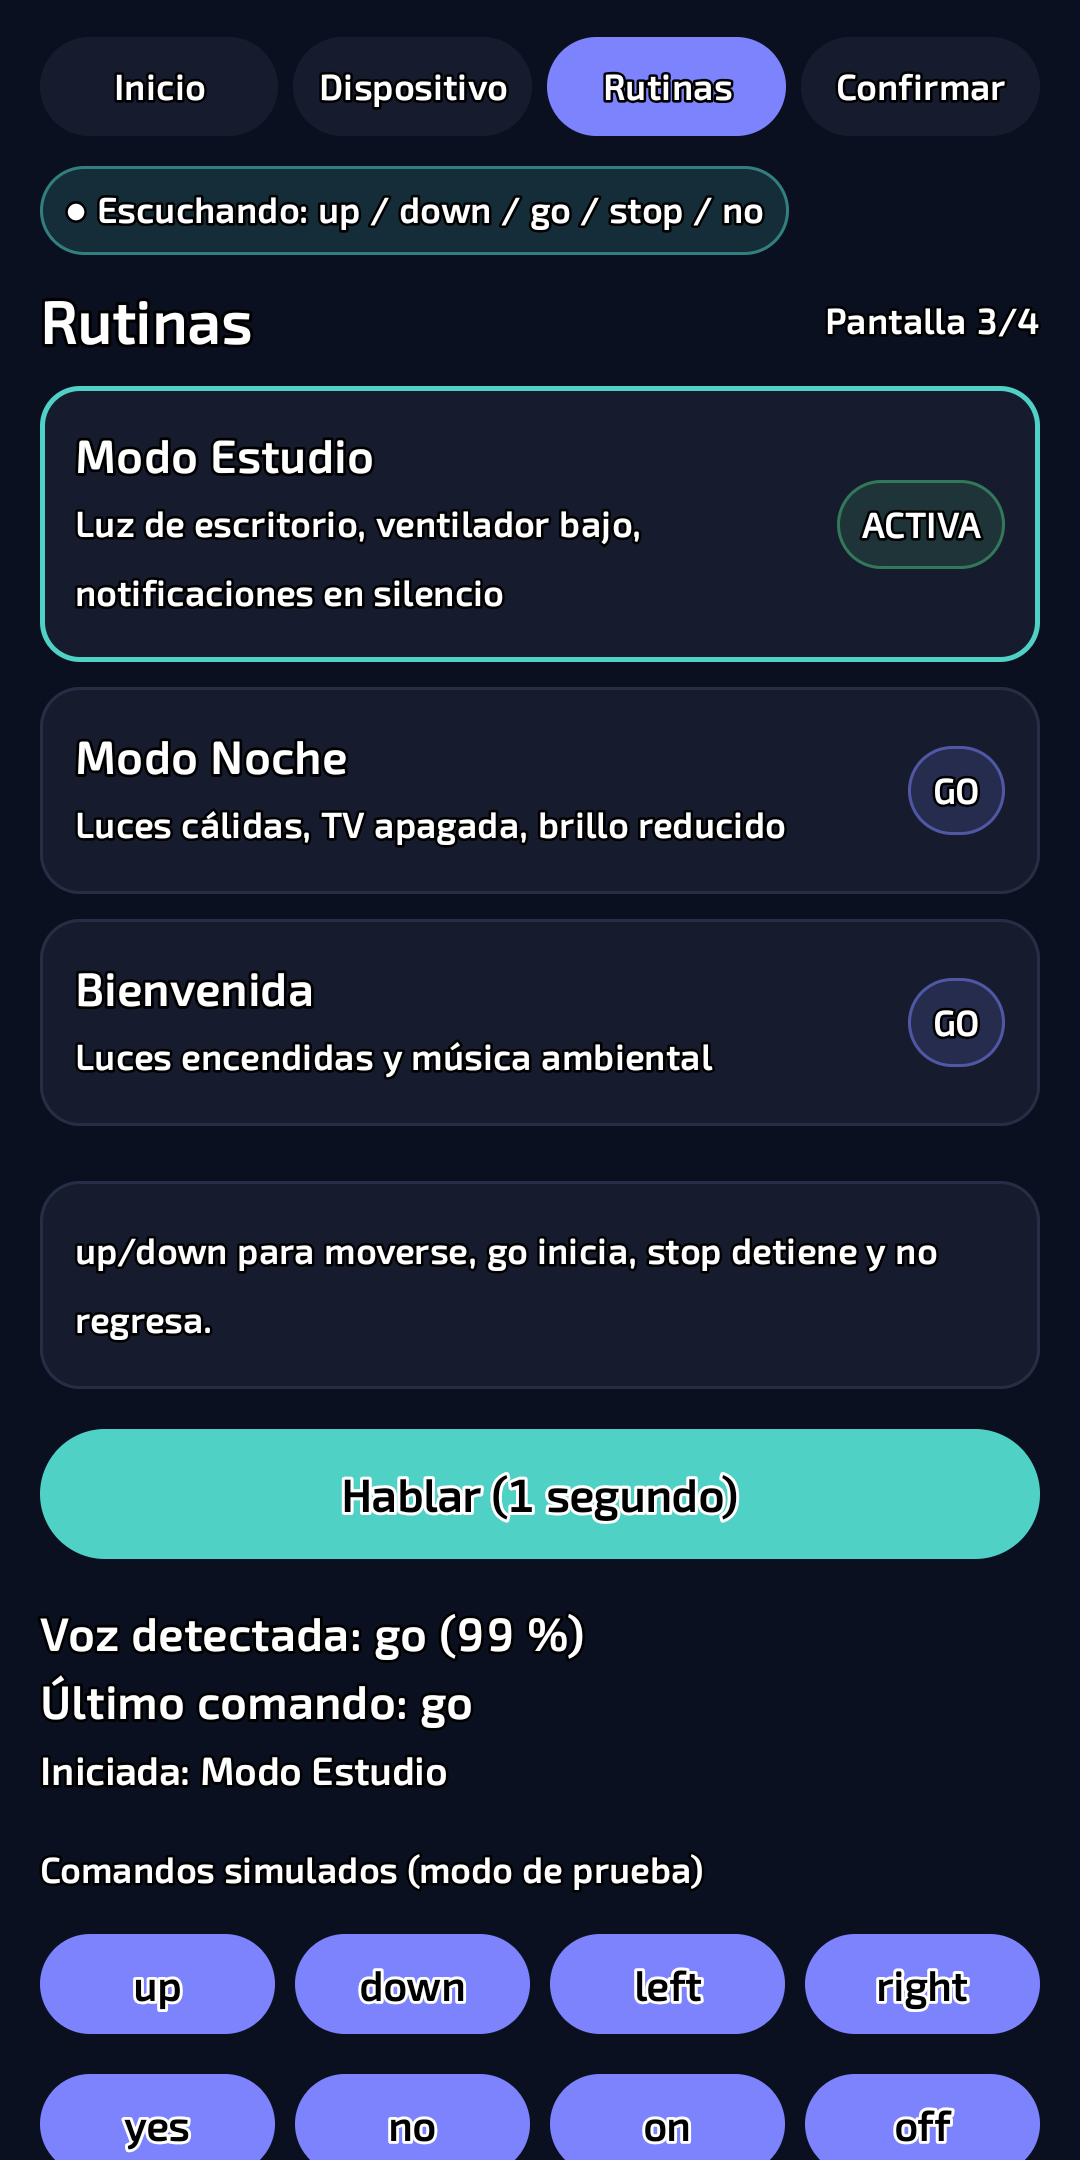
\includegraphics[width=\textwidth]{app_rutinas.png}\\[2pt]{\footnotesize (c) Rutinas}
\end{minipage}\hfill
\begin{minipage}[t]{0.23\textwidth}\centering
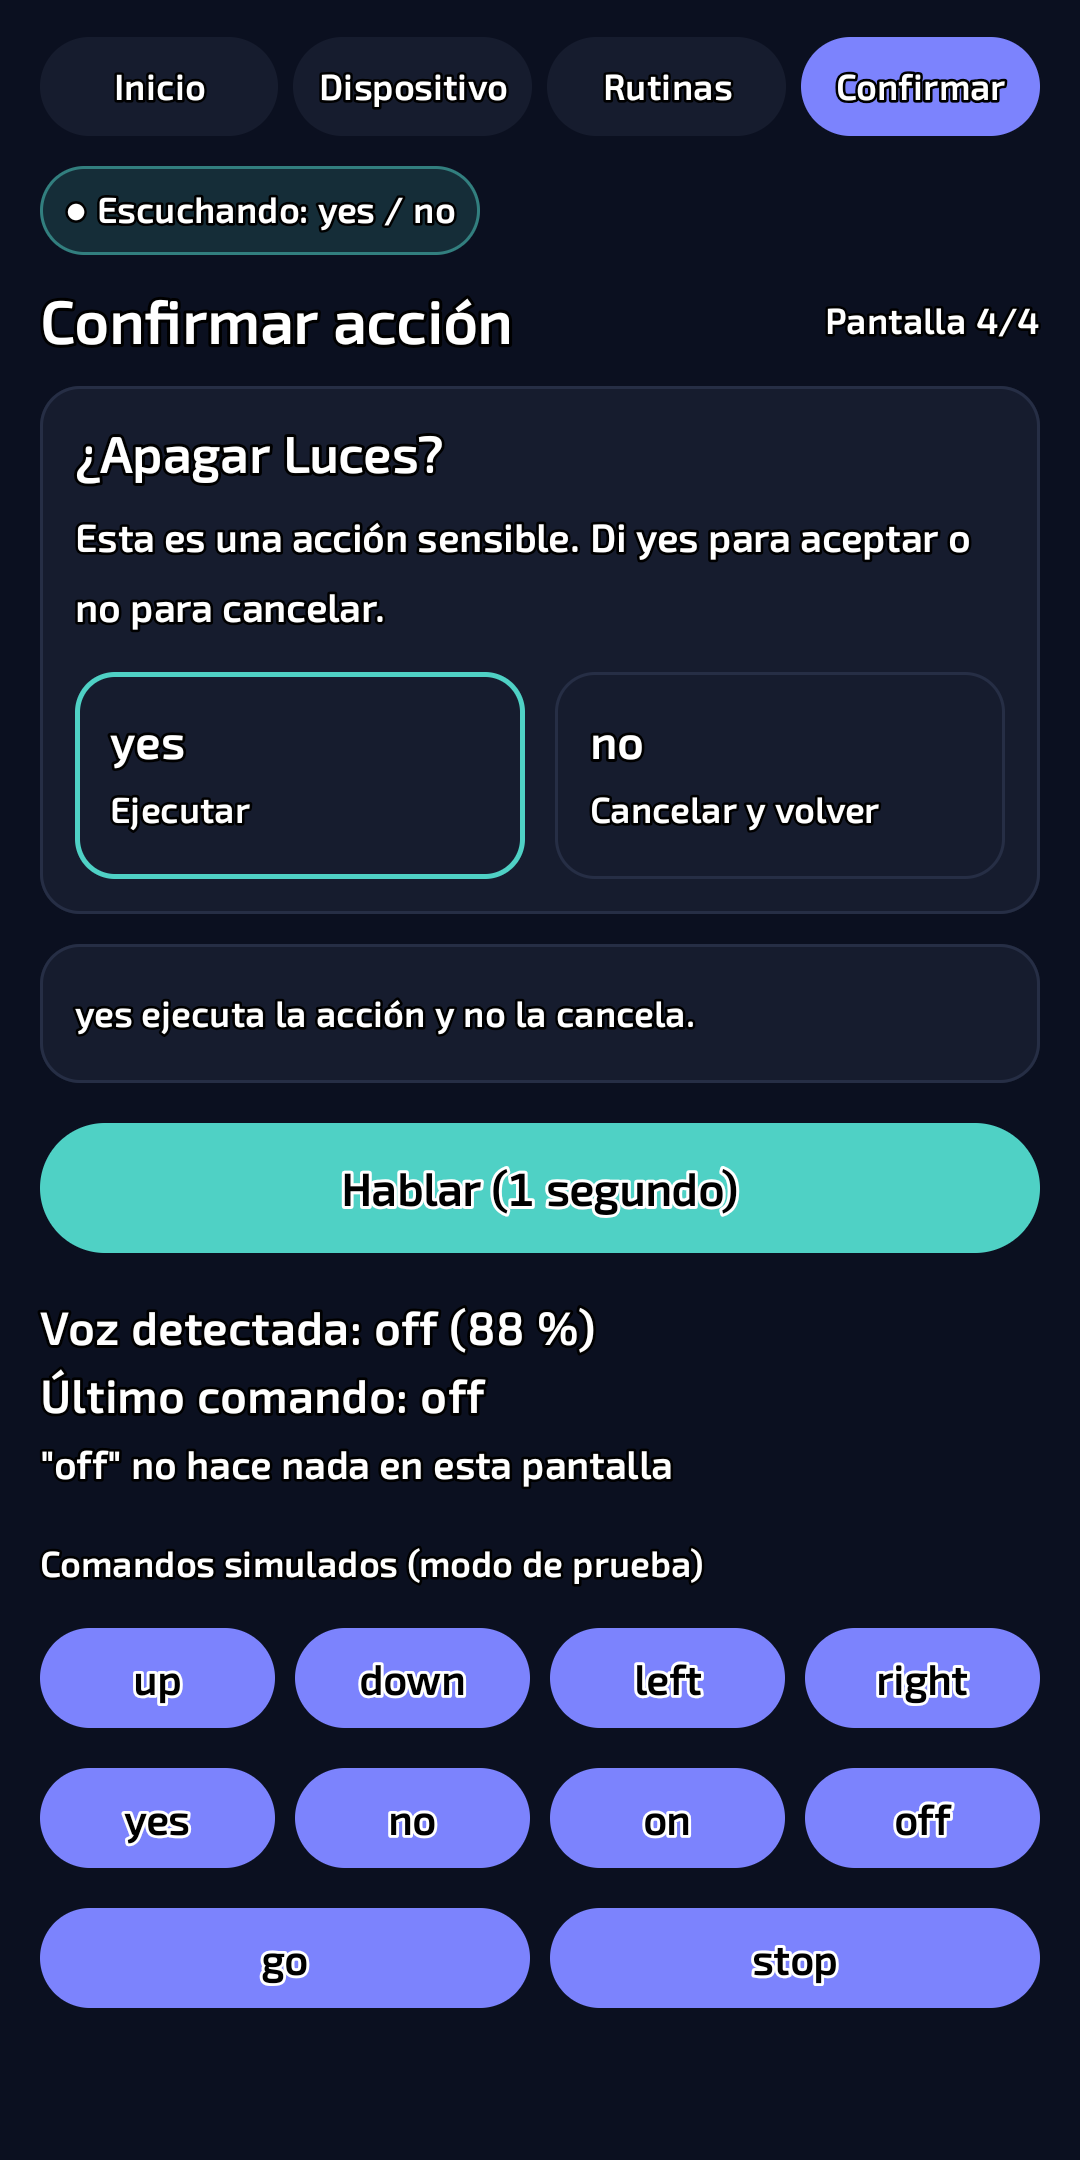
\includegraphics[width=\textwidth]{app_confirmacion.png}\\[2pt]{\footnotesize (d) Confirmación}
\end{minipage}
\caption{Pantallas de la aplicación en el Motorola Moto g54. Debajo del botón \textit{Hablar} se muestran la palabra detectada por el modelo, su confianza y la acción ejecutada; por ejemplo, en (c) el comando ``go'' con 99\,\% de confianza inició la rutina Modo Estudio, y en (d) el comando ``off'' se ignora porque en la pantalla de confirmación solo son válidos ``yes'' y ``no''.}
\label{fig:app}
\end{figure*}

\subsection{Pipeline de inferencia}
\begin{enumerate}
  \item El usuario toca el botón \textit{Hablar}. La primera vez, la aplicación solicita el permiso de micrófono.
  \item Se graba 1 segundo de audio con \texttt{AudioRecord}: mono, 16\,kHz, PCM de 16 bits.
  \item Cada muestra se divide entre 32\,768 para llevarla a $[-1, 1]$, igual que en el entrenamiento, y se forma el tensor $[16000]$.
  \item ONNX Runtime ejecuta el modelo y devuelve los 10 logits.
  \item Se aplica \textit{softmax} y se toma el comando con mayor probabilidad.
  \item Si la confianza es de al menos 70\,\%, se llama a \texttt{handle(comando)}. Si no, no se ejecuta ninguna acción.
  \item La pantalla muestra siempre el comando detectado y su confianza.
\end{enumerate}

La grabación y la inferencia se ejecutan en un hilo secundario para no congelar la interfaz.

\subsection{Problemas durante el desarrollo}
El modelo exportado venía en dos archivos, el \texttt{.onnx} con el grafo y un \texttt{.onnx.data} con los pesos. Para cargarlo desde la carpeta de recursos de la aplicación hubo que unirlos en un solo archivo de 3\,MB, y desde la versión corregida se exporta así directamente. Los otros dos problemas fueron más simples. Al separar el código en cuatro archivos quedó una copia vieja de \texttt{MainActivity.kt} con todas las clases adentro, y el compilador lanzaba errores de \textit{Redeclaration} hasta que la borramos. En otro momento, al pegar código, terminó texto de Kotlin dentro del \texttt{AndroidManifest.xml} y el proyecto dejó de compilar hasta reemplazar el archivo.

\subsection{Prueba en el dispositivo}
La aplicación se probó en un Motorola Moto g54 5G (Android 14), repitiendo cada comando 5 veces (Tabla~\ref{tab:prueba}). La hizo uno de los autores, hablante nativo de español; como el dataset está grabado sobre todo por angloparlantes, el acento puede influir en las confianzas más bajas.

\begin{table}[htbp]
\caption{Prueba en el dispositivo (5 intentos por comando)}
\label{tab:prueba}
\centering
\resizebox{\columnwidth}{!}{%
\begin{tabular}{lccc}
\toprule
Comando & Reconocidos & Ejecutados ($\geq$70\,\%) & Confianza media$^{*}$ \\
\midrule
yes   & 5/5 & 5/5 & 99.8\,\% \\
no    & 5/5 & 4/5 & 74.6\,\% \\
up    & 5/5 & 3/5 & 77.6\,\% \\
down  & 5/5 & 5/5 & 98.6\,\% \\
left  & 5/5 & 4/5 & 86.4\,\% \\
right & 5/5 & 5/5 & 99.0\,\% \\
on    & 5/5 & 5/5 & 98.2\,\% \\
off   & 4/5 & 2/5 & 70.8\,\% \\
stop  & 5/5 & 5/5 & 98.4\,\% \\
go    & 5/5 & 5/5 & 94.8\,\% \\
\midrule
Total & 49/50 (98\,\%) & 43/50 (86\,\%) & 90.2\,\% \\
\bottomrule
\end{tabular}}

\vspace{2pt}
\parbox{\columnwidth}{\footnotesize $^{*}$Promedio de la confianza en los intentos donde se detectó la palabra correcta.}
\end{table}

La palabra correcta apareció en 49 de los 50 intentos y 43 superaron el umbral. De los 7 descartados, 6 eran detecciones correctas con poca confianza: dos de ``up'', dos de ``off'', uno de ``no'' y uno de ``left''. El séptimo fue el único error de la prueba, un ``off'' que el modelo tomó como ``up'' con 62\,\% de confianza. Como no llegó al umbral, la aplicación no hizo nada, y en toda la prueba no hubo acciones incorrectas.

``No'', ``up'' y ``off'', las palabras con confianza más baja en el teléfono, también están entre las de menor exactitud en test, y ``off''$\rightarrow$``up'' es una de las confusiones que aparecen en la Fig.~\ref{fig:confusion}. Con el umbral en 70\,\%, esos 6 comandos correctos habrían tenido que repetirse.

\section{Limitaciones}
\begin{itemize}
  \item La prueba en el dispositivo se hizo con un solo hablante, en un ambiente silencioso y con 5 repeticiones por comando. Es una muestra pequeña e indicativa.
  \item La aplicación graba exactamente 1 segundo desde que se toca el botón. Si el usuario habla tarde, la palabra puede quedar cortada.
  \item El modelo siempre elige uno de los 10 comandos; no tiene una clase de ``silencio'' o ``palabra desconocida''. El umbral de 70\,\% reduce las acciones incorrectas, pero no las elimina.
  \item La división del dataset fue aleatoria por audio, por lo que un mismo hablante puede aparecer en entrenamiento y en prueba. Esto puede hacer que la exactitud en test sea algo optimista.
\end{itemize}

\section{Conclusiones}
Construimos el sistema completo, desde el preprocesamiento del audio hasta una aplicación Android que reconoce los 10 comandos sin conexión a internet.

El modelo de la aplicación es LeNet-5 entrenado con SpecAugment, con 92.2\,\% de exactitud en test. El aumento de datos le sirvió a LeNet-5 porque frenó el sobreajuste, pero a MobileNet lo perjudicó: con 14\,000 parámetros y las mismas épocas ya le costaba aprender, y las máscaras le complicaron más la tarea. Aun así, MobileNet quedó solo 3.4 puntos por debajo con 52 veces menos parámetros, y sería la mejor opción si la aplicación tuviera que escuchar de forma continua o correr en un teléfono más limitado.

Los errores del modelo se concentran en pocos pares de palabras, sobre todo ``no''/``go'' y ``off''/``on''/``up''. En el teléfono reconoció 49 de 50 comandos, y el único error no se ejecutó porque quedó por debajo del umbral.

Meter el preprocesamiento dentro del ONNX simplificó la aplicación, pero un error en la celda de exportación produjo un modelo que cargaba bien y no reconocía nada. Comparar las salidas de PyTorch y de ONNX sobre audios reales debió ser parte del proceso desde el principio.

Como trabajo futuro quedan entrenar MobileNet por más épocas, agregar clases de ``silencio'' y ``palabra desconocida'', dividir el dataset por hablante y permitir la escucha continua.

\begin{thebibliography}{00}

\bibitem{lecun1998} Y. LeCun, L. Bottou, Y. Bengio y P. Haffner, ``Gradient-based learning applied to document recognition,'' \textit{Proceedings of the IEEE}, vol. 86, no. 11, pp. 2278--2324, 1998.

\bibitem{howard2017} A. G. Howard \textit{et al.}, ``MobileNets: Efficient convolutional neural networks for mobile vision applications,'' \textit{arXiv preprint arXiv:1704.04861}, 2017.

\bibitem{park2019} D. S. Park, W. Chan, Y. Zhang, C.-C. Chiu, B. Zoph, E. D. Cubuk y Q. V. Le, ``SpecAugment: A simple data augmentation method for automatic speech recognition,'' \textit{arXiv preprint arXiv:1904.08779}, 2019.

\bibitem{warden2018} P. Warden, ``Speech Commands: A dataset for limited-vocabulary speech recognition,'' \textit{arXiv preprint arXiv:1804.03209}, 2018.

\bibitem{sainath2015} T. N. Sainath y C. Parada, ``Convolutional neural networks for small-footprint keyword spotting,'' en \textit{Proc. Interspeech}, 2015, pp. 1478--1482.

\bibitem{zhang2017} Y. Zhang, N. Suda, L. Lai y V. Chandra, ``Hello Edge: Keyword spotting on microcontrollers,'' \textit{arXiv preprint arXiv:1711.07128}, 2017.

\bibitem{sandler2018} M. Sandler, A. Howard, M. Zhu, A. Zhmoginov y L.-C. Chen, ``MobileNetV2: Inverted residuals and linear bottlenecks,'' en \textit{Proc. IEEE Conf. Computer Vision and Pattern Recognition (CVPR)}, 2018, pp. 4510--4520.

\bibitem{tang2018} R. Tang y J. Lin, ``Deep residual learning for small-footprint keyword spotting,'' en \textit{Proc. IEEE Int. Conf. Acoustics, Speech and Signal Processing (ICASSP)}, 2018, pp. 5484--5488.

\bibitem{choi2019} S. Choi, S. Seo, B. Shin, H. Byun, M. Kersner, B. Kim, D. Kim y S. Ha, ``Temporal convolution for real-time keyword spotting on mobile devices,'' en \textit{Proc. Interspeech}, 2019, pp. 3372--3376.

\bibitem{kim2021} B. Kim, S. Chang, J. Lee y D. Sung, ``Broadcasted residual learning for efficient keyword spotting,'' en \textit{Proc. Interspeech}, 2021, pp. 4538--4542.

\bibitem{berg2021} A. Berg, M. O'Connor y M. T. Cruz, ``Keyword Transformer: A self-attention model for keyword spotting,'' en \textit{Proc. Interspeech}, 2021, pp. 4249--4253.

\bibitem{davis1980} S. Davis y P. Mermelstein, ``Comparison of parametric representations for monosyllabic word recognition in continuously spoken sentences,'' \textit{IEEE Trans. Acoustics, Speech, and Signal Processing}, vol. 28, no. 4, pp. 357--366, 1980.

\bibitem{nair2010} V. Nair y G. E. Hinton, ``Rectified linear units improve restricted Boltzmann machines,'' en \textit{Proc. Int. Conf. Machine Learning (ICML)}, 2010, pp. 807--814.

\bibitem{ko2015} T. Ko, V. Peddinti, D. Povey y S. Khudanpur, ``Audio augmentation for speech recognition,'' en \textit{Proc. Interspeech}, 2015, pp. 3586--3589.

\bibitem{onnxruntime} ONNX Runtime developers, ``ONNX Runtime,'' 2024. [En línea]. Disponible en: \url{https://onnxruntime.ai}

\end{thebibliography}

\end{document}